%%%%%%%%%%%%%%%%%%%%%%%%%%%%%%%%%%%%%%%%%%%%%%%
%%%This is a science homework template. Modify the preamble to suit your needs. 
%The junk text is   there for you to immediately see how the headers/footers look at first 
%typesetting.

\documentclass[12pt]{article}

%AMS-TeX packages
\usepackage{amssymb,amsmath,amsthm, mathtools} 
\usepackage{commath}
\usepackage[margin=1in]{geometry}
\usepackage{graphicx,ctable,booktabs}
\usepackage[retainorgcmds]{IEEEtrantools}
\usepackage{cancel}
\usepackage{wrapfig}
\usepackage{braket}
\usepackage{enumitem}
\usepackage{pdfpages}
\usepackage{subcaption}
\usepackage{xurl}

\usepackage{graphicx}
\usepackage{subfig}

%Redefining sections as problems

\makeatletter
\newenvironment{problem}{\@startsection
	{section}
	{1}
	{-.2em}
	{-3.5ex plus -1ex minus -.2ex}
	{2.3ex plus .2ex}
	{\pagebreak[3]%forces pagebreak when space is small; use \eject for better results
		\large\bf\noindent{Problem }
	}
}
{%\vspace{1ex}\begin{center} \rule{0.3\linewidth}{.3pt}\end{center}}
	\begin{center}\large\bf \ldots\ldots\ldots\end{center}}
\makeatother

%Fancy-header package to modify header/page numbering 

\usepackage{fancyhdr}
\pagestyle{fancy}
\lhead{Problem \thesection}
\chead{} 
\rhead{\thepage} 
\lfoot{\small\scshape PHYS 600} 
\cfoot{} 
\rfoot{\footnotesize HW 4} 
\renewcommand{\headrulewidth}{.3pt} 
\renewcommand{\footrulewidth}{.3pt}
\setlength\voffset{-0.25in}
\setlength\textheight{648pt}
\allowdisplaybreaks

\newcommand{\partder}[3]{\ensuremath{\left(\frac{\partial {#1}}{\partial {#2}}\right)_{#3}}}

\newcommand{\braks}[1]{\ensuremath{\left\langle{#1} \right\rangle} }

\newcommand{\Omx}[1]{\ensuremath{\Omega_\mathrm{#1} } }
\newcommand{\rhox}[1]{\ensuremath{\rho_\mathrm{#1} } }

\setlength{\parindent}{0pt} % No indent by default

%%%%%%%%%%%%%%%%%%%%%%%%%%%%%%%%%%%%%%%%%%%%%%%

%
%Contents of problem set
%    

\begin{document}
	
	\title{PHYS 600: Homework 4}
	\author{Yarone Tokayer}
	\date{October 29, 2023}
	
	\maketitle
	
	\thispagestyle{empty}

	\begin{problem}{Recombination}
		\begin{enumerate}
			\item The process we are interested in here is recombination of protons and electrons into neutral hydrogen.  i.e., the reaction \begin{equation*}
				e^- + p^+ \leftrightarrow \mathrm{H} + \gamma
			\end{equation*} tending to the right as the Universe cools.  Recombination occurred at $z\sim 1100$ (around the redshift of the CMB), so we can treat the species as non-relativistic.  We then have, for each species of interest, $i$, \begin{align*}
				n_i &= g_i \left(\frac{m_i T}{2\pi}\right)^{3/2}e^\frac{\mu_i-m_i}{T}
			\end{align*} where $T$ is the temperature of the baryon-photon fluid with which these particles are all in equilibrium.  In order to eliminate chemical potential from the equation, we evaluate: \begin{align}
				\frac{n_\mathrm{H}}{n_en_p} &= \frac{g_\mathrm{H}}{g_eg_p} \left( \frac{m_\mathrm{H}}{m_em_p} \frac{ 2\pi}{T}\right)^{3/2} e^\frac{\cancel{\mu_\mathrm{H}} - \cancel{(\mu_e+\mu_p)} - m_\mathrm{H} + m_e + m_p}{T} \notag
				\\
				\implies \frac{n_\mathrm{H}}{n_e^2} &= \left( \frac{m_\mathrm{H}}{m_em_p} \frac{ 2\pi}{T}\right)^{3/2} e^{E_I/T} \notag
				\\
				&= \left( \frac{ 2\pi}{m_eT}\right)^{3/2} e^{E_I/T}  \label{eq:n_h/n_e^2}
			\end{align} where we have used the fact that $\mu_\mathrm{H} = \mu_e + \mu_p$, $g_\mathrm{H} = 4$, $m_p\approx m_\mathrm{H}$, $g_e = g_p = 2$, $m_e + m_p - m_\mathrm{H} = 13.6 \text{ eV} \equiv E_I$ (the ionization energy of hydrogen), and $n_e = n_p$ in a neutral universe.\\
			
			Now, we shift our focus to finding an expression for $X_e$, the free electron fraction defined by $X_e \equiv n_e/(n_p + n_\mathrm{H})$.  If we assume that protons and hydrogen comprises all of the baryons in the Universe at this point (i.e., we ignore the abundance of helium), then we have \begin{align*}
				n_p + n_\mathrm{H} = n_b &= \eta n_\gamma
				\\
				&= \eta \frac{\zeta(3)}{\pi^2}2 T^3
			\end{align*} where $\eta$ is the baryon-to-photon ratio, we have made use of the number density formula for relativistic species, and the fact that $g_\gamma = 2$.  But now we can make use of Eq.~\ref{eq:n_h/n_e^2} and write: \begin{align*}
				\frac{1 - X_e}{X_e^2} &= \frac{(1 - n_e) n_b}{n_e^2}
				\\
				&= \frac{n_\mathrm{H}}{n_e^2}n_b
				\\
				&=\frac{2\zeta(3)}{\pi^2} \eta  \left(  \frac{ 2\pi T}{m_e}\right)^{3/2} e^{E_I/T},
			\end{align*} the Saha equation.
			
			\item The Saha equation is a quadratic equation for $X_e$ of the form $AX_e + BX_e + C = 0$, with $B = 1$, $C=-1$, and \begin{equation*}
				A= \frac{2\zeta(3)}{\pi^2} \eta  \left(  \frac{ 2\pi T}{m_e}\right)^{3/2} e^{E_I/T}.
			\end{equation*} We then have, from the quadratic formula \begin{align*}
				X_e &= \frac{-1 \pm \sqrt{1 + 4A}}{2A}
			\end{align*} and we choose the $+$ sign, since $X_e$ must be a real number and $A > 0$ for all $T$.\\
			
			To get our expression to be in terms of $z$, we use the relation $T = T_0 (1+z)$, where $T_0$ is the temperature of the CMB today.  See Fig.~\ref*{fig:x_e}.  The code to generate this plot can be found in the appendix.
			
			\begin{figure}
				\centering
				\fbox{
					\begin{minipage}{\linewidth}
						\centering
						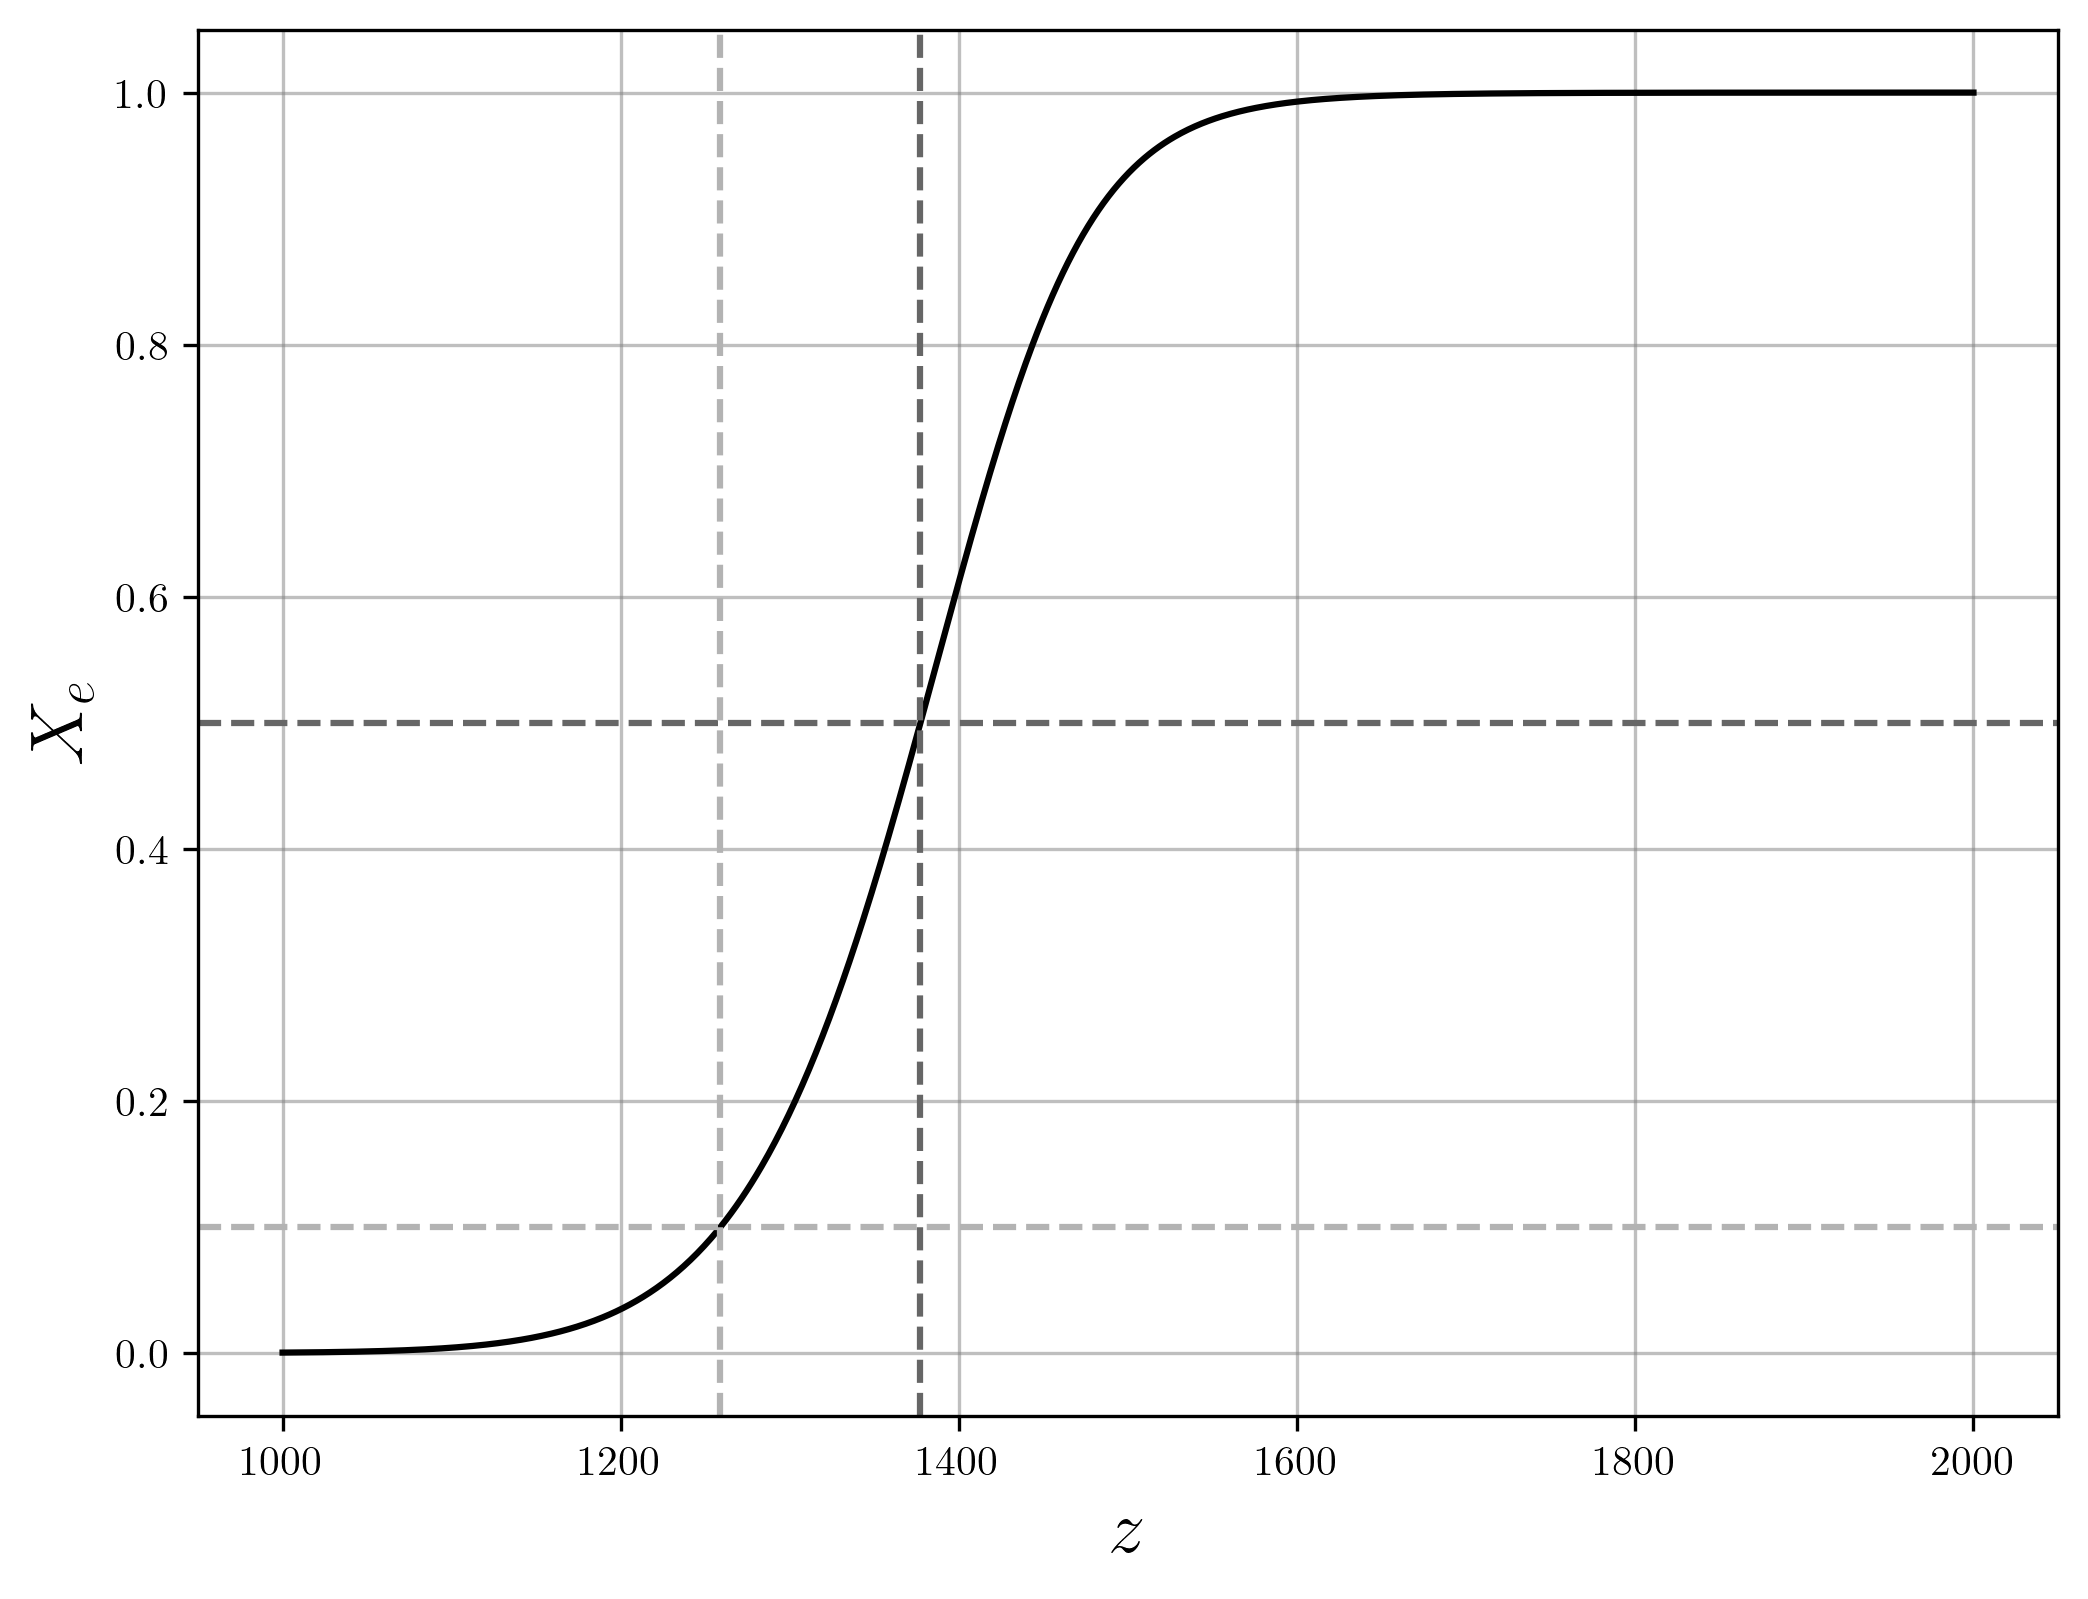
\includegraphics[width=0.65\linewidth]{x_e_plot.png}
						\caption{The free electron fraction as a function of redshift around the epoch of reionization.  The redshifts at which $X_e$ = 0.1 and 0.5 are indicated.}\label{fig:x_e}
					\end{minipage}
				}
			\end{figure}
			
			\item We use a bisection method to invert our function $X_e(z)$.  See the appendix.  We find that $\boxed{z(X_e = 0.1) \approx 1259}$ and $\boxed{z(X_e = 0.5) \approx 1377}$.  As can be seen from the plot, the transition from a universe with almost all free electrons free to one in which there are almost none are happens over a relatively short span of redshifts.
			
			\item For a single component universe, we have (see lecture notes) \begin{align*}
				t &= \frac{1}{H_0}\frac{2}{3(1  + w)}a^{\frac{3}{2}(1+w)}
				\\
				&= \frac{1}{H_0}\frac{2}{3(1  + w)}\left(\frac{1}{1+z}\right)^{\frac{3}{2}(1+w)}
			\end{align*} For matter, $w\approx 0$, and we get that $\boxed{t(z=1259)\approx 208,000 \text{ years}}$ (for $h=0.7$).
			
			\item We seek to solve \begin{align*}
				\Gamma_T(z) &= H(z)
				\\
				n_e(z)\sigma_T &= H_0 \sqrt{\Omx{m,0}( 1 + z )^3} & \text{(matter domination)}
				\\
				X_e(z)n_b(z)\sigma_T &= H_0 \sqrt{\Omx{m,0}( 1 + z )^3}
				\\
				X_e(z) \eta \frac{\zeta(3)}{\pi^2}2 T_0^3 (1+z)^3\sigma_T &= H_0 \sqrt{\Omx{m,0}( 1 + z )^3} & \text{($n_b$ formula above)}
				\\
				\implies X_e(z) (1+z)^{3/2} &= \frac{H_0\pi^2\sqrt{\Omx{m,0}}}{2\eta\zeta(3)\sigma_TT_0^3}
				\\
				&\approx 215.592 & \text{(see calculation in appendix)}
			\end{align*} We use a numerical bisection method to invert this equation for $z$ and we find that $\boxed{z_\mathrm{dec} \approx 1114}$.\\
			
			Using the same calculations as above, we get $\boxed{t_\mathrm{dec}\approx 250,000 \text{ years }}$ and $X_e(z_\mathrm{dec})\approx \boxed{0.0058}$.  In the words of Baumann, ``a large degree of neutrality is necessary before the universe becomes transparent to photons.''

		\end{enumerate} 
	\end{problem}
	
	\begin{problem}{``What-if'' BBN}

	\begin{itemize}
		\item Here, instead of the combination of protons and electrons into hydrogen, we consider the decay of neutrons into protons: \begin{align*}
			n + \nu_e \leftrightarrow p^+ + e^-
			\\
			n + e^+ \leftrightarrow p^+ + \bar{\nu}_e.
		\end{align*}  As before, we have for each species, \begin{align*}
			n_i &= g_i \left(\frac{m_i T}{2\pi}\right)^{3/2}e^\frac{\mu_i-m_i}{T}
		\end{align*}  Assuming that the chemical potentials of electrons and neutrinos are negligible, and using the face that $g_n = g_p$, we have \begin{align*}
			\frac{n_n}{n_p} &= \left(\frac{m_n}{m_p}\right)^{3/2}e^\frac{-(m_n - m_p)}{T}
			\\
			&\approx e^\frac{-(m_n - m_p)}{T}
			\\
			&\equiv e^{-\frac{Q}{T}},
		\end{align*} where we have approximated $m_n/m_p\approx 1$, and defined $Q\equiv m_n - m_p$.\\
		
		Defining the neutron fraction $X_n \equiv n_n/(n_n + n_p)$, we have \begin{align*}
			X_n^{-1} &= \frac{n_n}{n_n} + \frac{n_p}{n_n}
			\\
			&= 1 +  e^{\frac{Q}{T}}
			\\
			\implies X_n &= \frac{1}{1 +  e^{\frac{Q}{T}}}
			\\
			&= \frac{ e^{-\frac{Q}{T}}}{1 +  e^{-\frac{Q}{T}}}.
		\end{align*}
		
		\item For a freezeout temperature of $0.8$ MeV, we get a freezeout abundance of $\sim \boxed{0.16}$.  See appendix for the calculation.
		
		\item If every two neutrons ends up in a helium-4 atom, then \begin{align*}
			Y_P &= \frac{4n_\mathrm{He}}{n_\mathrm{H}}
			\\
			&= \frac{2n_n}{n_p}
			\\
			&= \frac{2n_n}{n_n + n_p}\frac{n_n + n_p}{n_p}
			\\
			&= \frac{2n_n}{n_n + n_p}\frac{n_n + n_p}{1 - n_n}
			\\
			&= \frac{2X_n}{1 - X_n}
			\\
			&\approx \boxed{ 0.39}.
		\end{align*}
		
		\item Here we perform the same calculations as above, but with $Q = -2.6$ MeV (double the actual difference).  We get $\boxed{X_n \approx 0.037}$ and $\boxed{Y_P\approx 0.078}$.
	\end{itemize}
		
	\end{problem}
	
	\begin{problem}{Freeze-in DM}
		\begin{enumerate}[label=(\alph*)]
			\item As instructed we begin with the Boltzmann equation for freeze-in: \begin{align*}
				\frac{1}{a^3} \frac{\dif}{\dif t} na^3 &= 2\Gamma h(t)n_\mathrm{\sigma,eq}(t)
			\end{align*} We define $Y\equiv n/T^3$, which implies that, for the LHS, \begin{align*}
				\frac{1}{a^3} \frac{\dif}{\dif t} na^3 &= \frac{T^3}{T_0^3} \frac{\dif}{\dif t} n\frac{T_0^3}{T^3}
				\\
				&= T^3 \frac{\dif Y}{\dif t}
				\\
				\implies \frac{\dif Y}{\dif t} &= 2\Gamma h(t)Y_\mathrm{\sigma,eq}(t)
			\end{align*} Now, to switch variables from $t$ to $x$, we note that the epoch of interest is radiation domination, during which $a\propto\sqrt{t}$.  Using the fact that $x\propto T^{-1} \propto a$, we have \begin{align*}
				\dif x \propto t^{-1/2}\dif t \propto x^{-1}\dif t \implies \frac{\dif}{\dif t} \propto x^{-1} \frac{\dif}{\dif x}
			\end{align*} So we have \begin{align*}
				x^{-1}\frac{\dif Y}{\dif x} &= \text{const.} \times 2\Gamma h(x)Y_\mathrm{\sigma,eq}(x)
				\\
				\implies \Aboxed{\frac{\dif Y}{\dif x}  &= \lambda_1 xh(x)Y_\mathrm{eq}(x)}
			\end{align*}
			
			\item First we need an expression for $Y_\mathrm{eq}(x)$.  In general for Fermions, we have the equilibrium numberpye density as \begin{align*}
				n &= \frac{g}{2\pi^2}T^3 I(x) & I(x) &= \int_0^\infty\dif\xi \frac{\xi^2}{\exp\left[\sqrt{\xi^2 + x^2}\right] +1}
			\end{align*}\begin{align*}
				\implies Y_\mathrm{eq} &= \frac{g}{2\pi^2} I(x)
			\end{align*}  Since we are looking for order of magnitude results, we can look at the case of $g=1$.  See plot in Fig.~\ref{fig:y}
			
			\begin{figure}[ht!]
				\centering
				\fbox{
					\begin{minipage}{\linewidth}
						\centering
						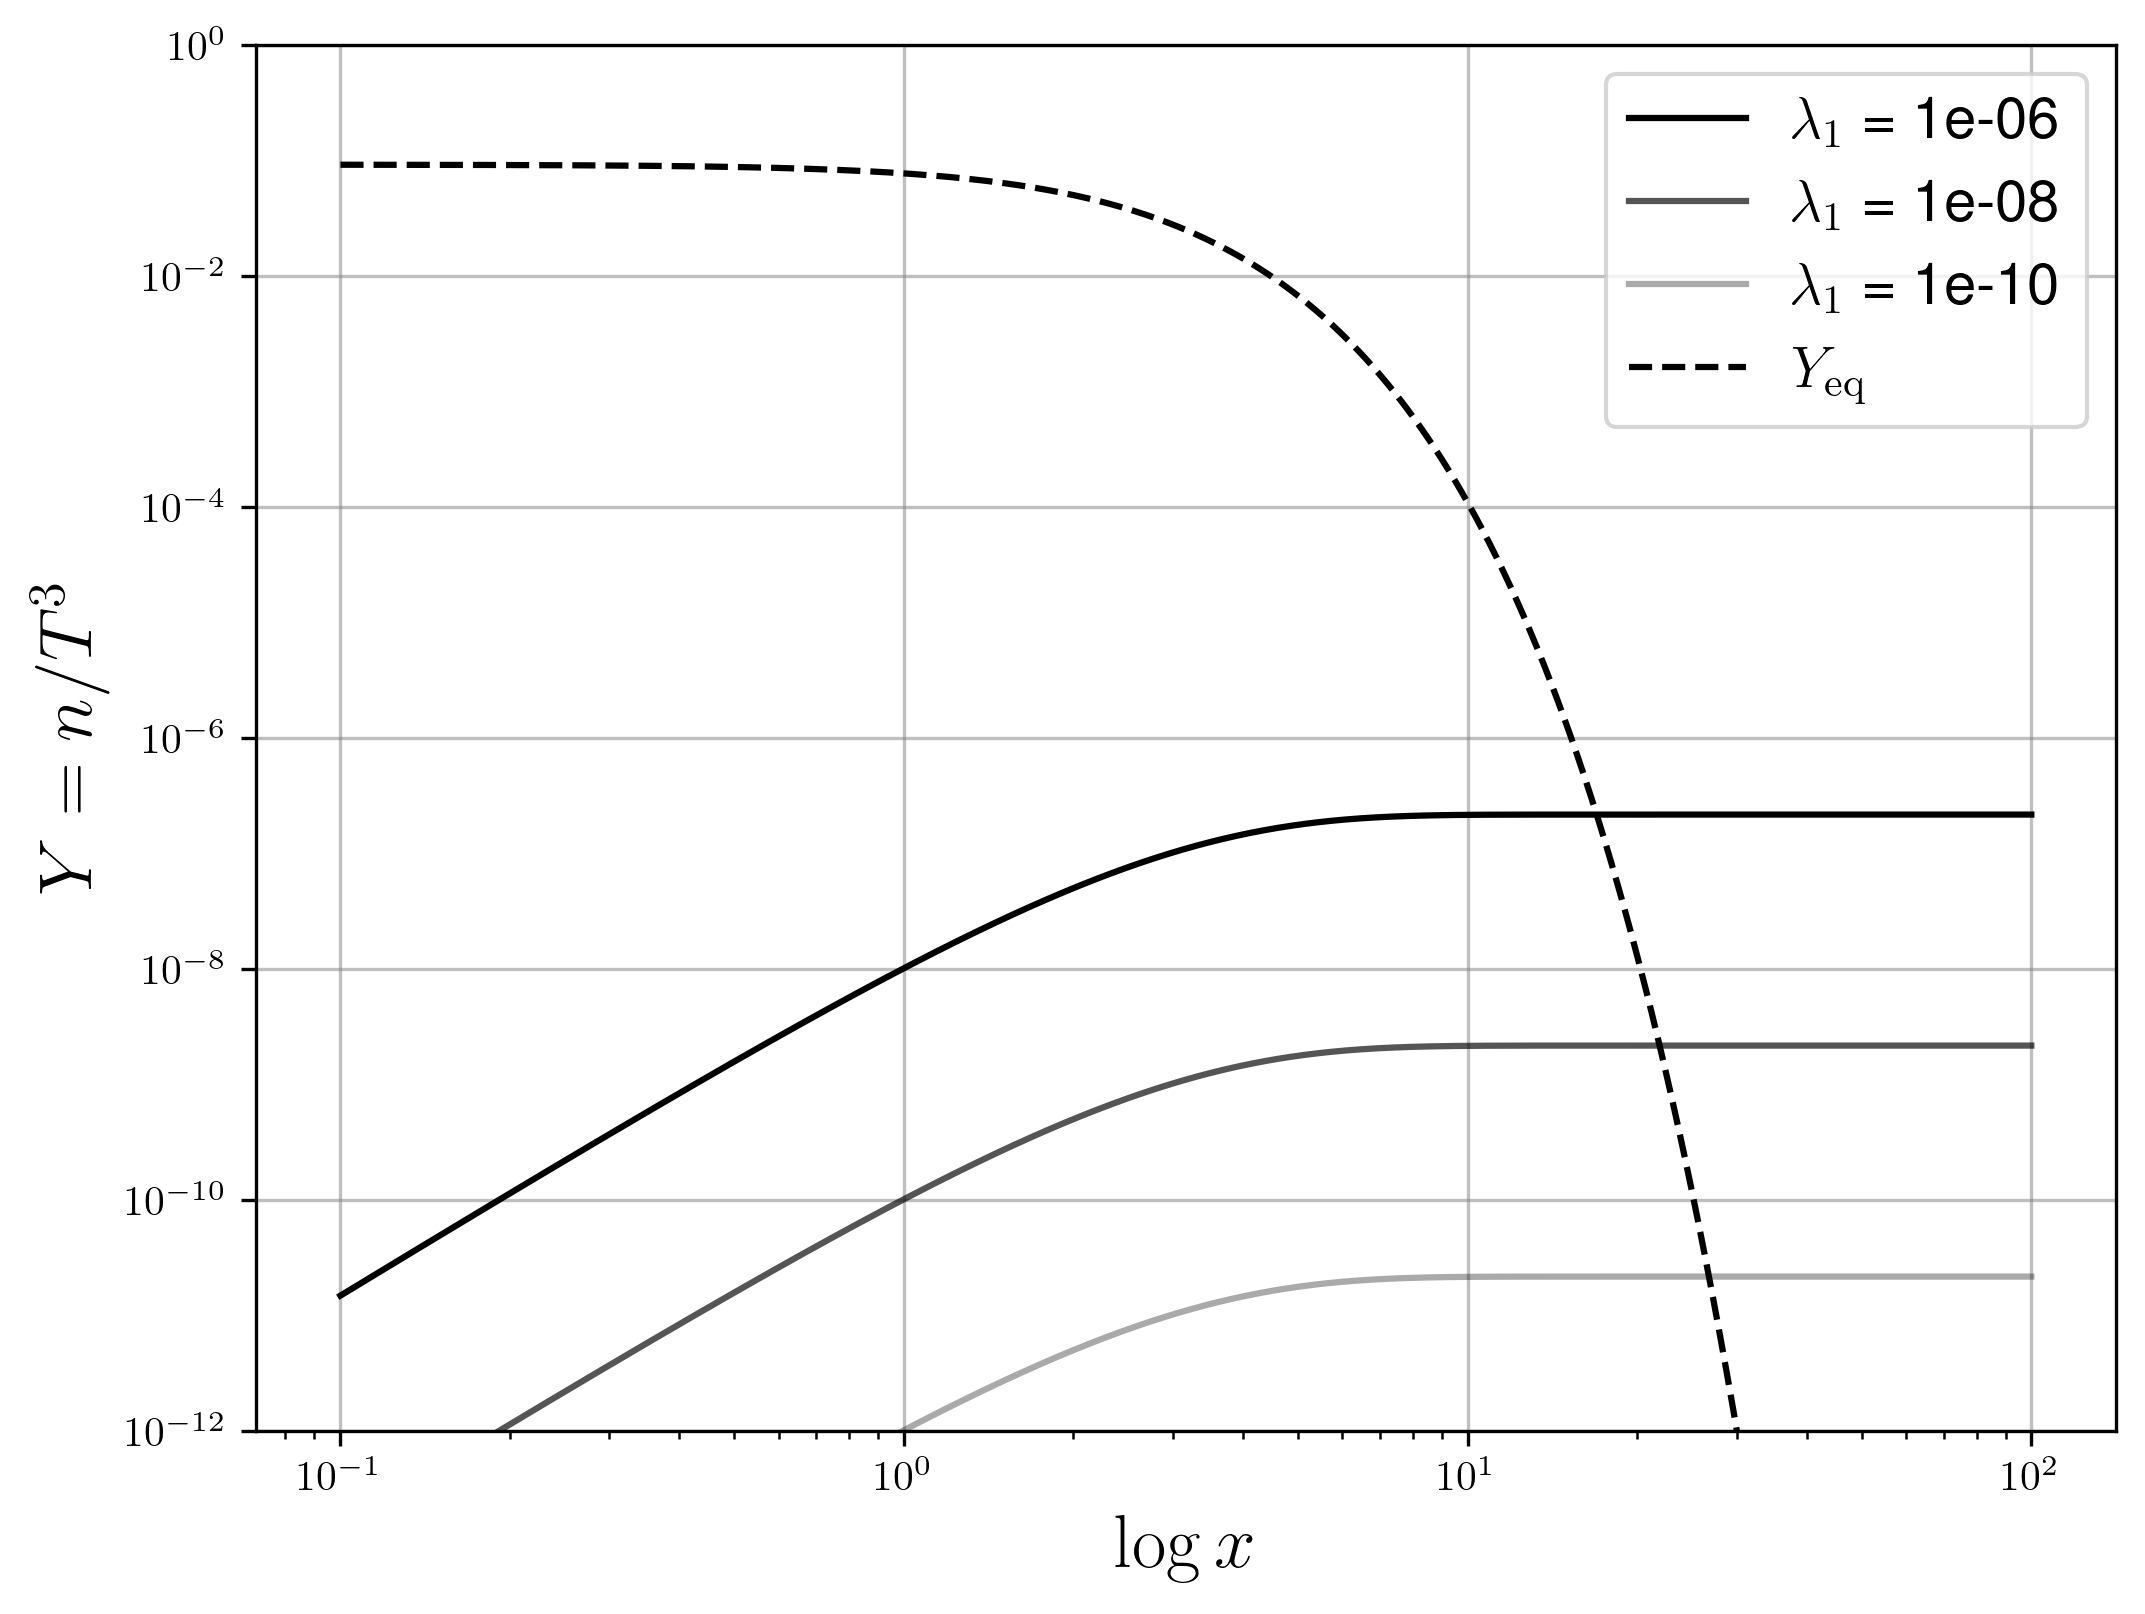
\includegraphics[width=0.65\linewidth]{y_plot.png}
						\caption{The free electron fraction as a function of redshift around the epoch of reionization.  The redshifts at which $X_e$ = 0.1 and 0.5 are indicated.}\label{fig:y}
					\end{minipage}
				}
			\end{figure}
			
			\item Notice that in the ``freeze in'' scenario, abundance \textit{decreases} with the interaction rate $\Gamma$, while in the ``freeze out'' scenario, the opposite is true.
			
		\end{enumerate}
	\end{problem}


% Appendix
\appendix
\section{Python code}
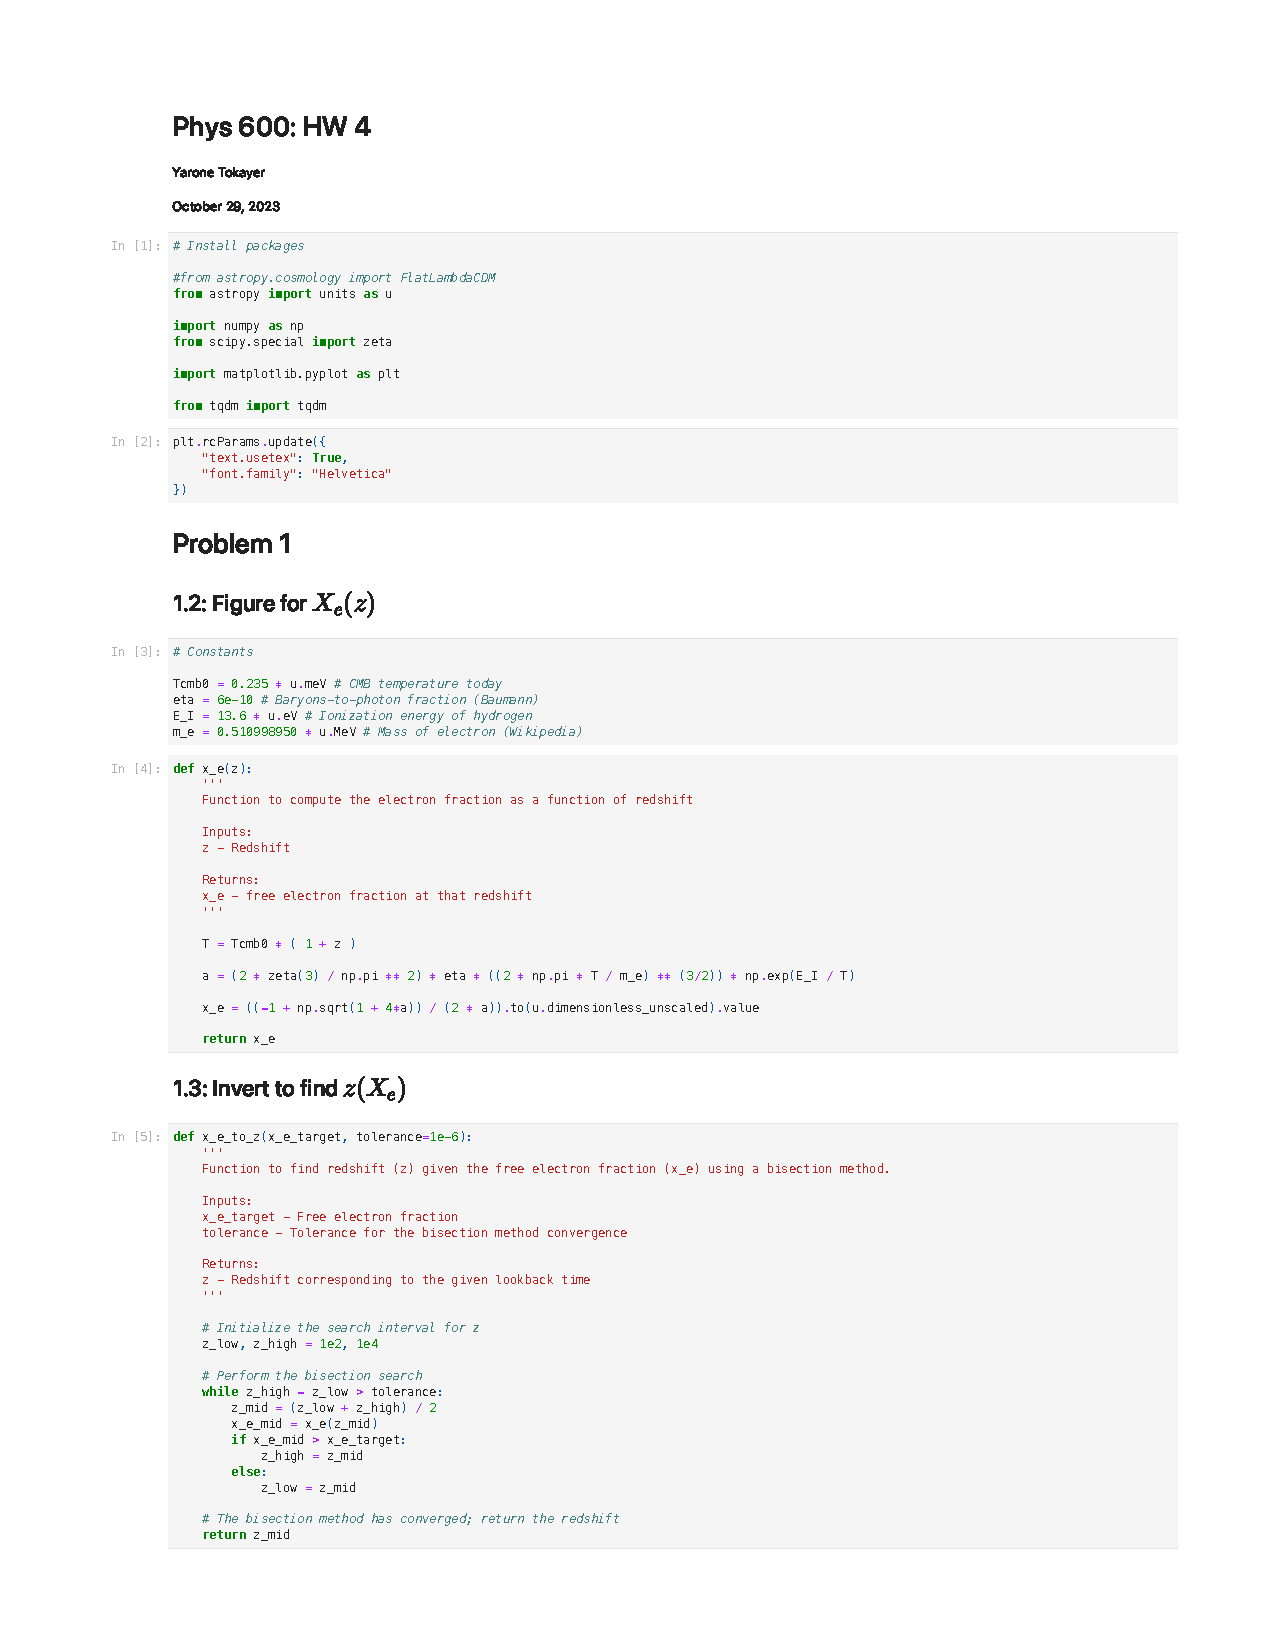
\includepdf[pages=-, frame=true, scale=0.9]{/Users/yaronetokayer/Yale Drive/Classes/PHYS 600/phys600 hw/phys600 hw 4/phys600 hw 4 work.pdf}



\end{document}